\documentclass[]{article}
\usepackage[a4paper, total={6.5in, 8.5in}]{geometry}
\usepackage{hyperref}
\usepackage{amsmath}
\usepackage{amssymb}
\usepackage{graphicx}
\usepackage{float}
\usepackage{algorithm}
\usepackage{algpseudocode}
\usepackage{color}

\title{Towards Comparable Active Learning}

\begin{document}

\maketitle

\section{Introduction}


\subsection{Contribution}

%%%%%%%%%%%%%%%%%%%%%%%%%%%%%%%%%%%%%%%%%%%%%%%%%%%%%%%%%%%%%%%%%%%%%%%%%%%%%%%%%%
\section{Related Work}
{\color{red} Version: Braindump}\\
Many different algorithms have been proposed for active learning. 
In this work we focus on those approaches that have shown consistent results over the years as well as newer approaches that have demonstrated significant lifts in their initial experiments.
AL algorithms can be categorized into two classes: Geometric approaches and uncertainty-based approaches.
Geometric approaches include CoreSet \cite{sener2017active} and TypiClust \cite{hacohen2022active}, which use clustering techniques to partition the data and then sample their unlabeled points based on the clusters.
Uncertainty-based approaches include classic uncertainty sampling (based on Shannon-Entropy and the margin-score), BALD \cite{kirsch2019batchbald} and BADGE \cite{ashdeep}, which use metrics to measure the classifiers state. \\ [1mm]
%
Some previous work also aimed to provide a benchmark suite for active learning:
The authors of \cite{beck2021effective} and \cite{li2022empirical} both focus on active learning in the image domain.
While \cite{beck2021effective} discuss a new metric to measure AL performance, which they call "Label Efficiency" and provide experiments on many common configurations for data preparation, model training and other hyperparameters, \cite{li2022empirical} focuses on combined approaches of AL and semi-supervised learning to aid model training.
The authors of \cite{hu2021towards} study models that are learned with AL techniques in the image and text domain.
They test for several different properties of the models including robustness, response to compression techniques and final performance.



%%%%%%%%%%%%%%%%%%%%%%%%%%%%%%%%%%%%%%%%%%%%%%%%%%%%%%%%%%%%%%%%%%%%%%%%%%%%%%%%%%
\section{Overview}
Table \ref{tab:benchmark_comparison} shows a feature comparison between our proposed benchmark and several existing benchmarks in the literature, as well as methodological AL papers with an extensive experiments section. \\
{\color{red} TODO} We include in this table any methodological paper that experiments on at least two domains. \\
{\color{red} TODO} Define AL scenarios (really hard)
\begin{table}[h]
	\centering
	\begin{tabular}{l | c c c c c}
		Paper & \# Datasets & Domains & Scenarios & Oracle & RL Alg. \\
		\hline
		Beck et al. \cite{beck2021effective} & 4 & 1 & 3 & - & - \\
		Hu et al. \cite{hu2021towards} & 5 & 2 & 1 & - & - \\
		Li et al. \cite{li2022empirical} & 5 & 1 & 1 & - & - \\
		\textbf{Ours} & 5 & 2 & 2 & \checkmark & -
	\end{tabular}
	\caption{Comparison of our benchmark with the existing literature}
	\label{tab:benchmark_comparison}
\end{table}


%%%%%%%%%%%%%%%%%%%%%%%%%%%%%%%%%%%%%%%%%%%%%%%%%%%%%%%%%%%%%%%%%%%%%%%%%%%%%%%%%%
\subsection{Problem Description / Delineation}
\textbf{Lars' Version} \\
Given
\begin{itemize}
	\item a number $B\in\mathcal{N}$ (called budget),
	\item two spaces $\mathcal{X}$ and $\mathcal{Y}$,  {\tiny e.g., $\mathcal{X}:=\mathcal{R}^M, \mathcal{Y}:=\mathcal{R}^T$},
	\item a sample $\mathcal{D}_1,\ldots,\mathcal{D}_N \subseteq (\mathcal{X}\times \mathcal{Y})^*$ of
	sequences of pairs $(x,y)$  from an unknown distribution $p$
	(called datasets),
	%  {\tiny with $|\mathcal{D}_n|\geq B$ for all $n\in 1{:}N$,}
	{\tiny with $p(\mathcal{D})=0$ for $|\mathcal{D}|<B$,}
	\item a function $\ell:\mathcal{Y}\times \mathcal{Y}\rightarrow \mathcal{R}$ (called loss), and
	\item a function $A:  (\mathcal{X} \times \mathcal{Y})^* \times \mathcal{X}^* \rightarrow \mathcal{Y}^{\mathcal{X}}$
	(called learning algorithm),
\end{itemize}
find a function
\begin{align*}
	a: (\mathcal{X}\times \mathcal{Y})^* \times \mathcal{X}^* \rightarrow \{0,1\}^*
	\quad\quad \text{\tiny (equivariant in the second argument)}
\end{align*}
% which is equivariant in the second argument, 
called acquisition function,
s.t. the expected loss of a model learned on
all predictors 
plus $B$ sequentially acquired
targets is minimal:
\begin{align*}
	\mathbb{E}_{\mathcal{D}\text{train},\mathcal{D}\text{test}\sim p}   &
	% \frac{1}{|\mathcal{D}\text{test}|} \sum_{(x,y)\in\mathcal{D}\text{test}}
	% \operatorname{avg} \{
	%  \ell(y, \hat y(x)) \mid (x,y)\in\mathcal{D}\text{test} \}
	\operatorname{avg}\limits_{(x,y)\in\mathcal{D}\text{test}}
	\ell(y, \hat y(x)) 
	\\
	\text{with }
	\hat y:= & A( (\mathcal{D}\text{train}_{n_1},\ldots,\mathcal{D}\text{train}_{n_B}), \mathcal{D}\text{train}|_{\mathcal{X}})
	\\ 
	n_b := & \text{index}( a( (\mathcal{D}\text{train}_{n_1},\ldots,\mathcal{D}\text{train}_{n_{b-1}}), \mathcal{D}\text{train}|_{\mathcal{X}}) ),
	\quad b\in 1{:}B
\end{align*}
\textbf{Notes:}
\begin{itemize}
	\item We would need to switch from lowest expected loss to highest AUC
	\item 
\end{itemize}
\vspace{5mm}
\textbf{Thorben's Version}\\
\textbf{Basic Classification}\\
We assume a dataset $\mathcal{D} := (x_i, y_i) \hspace{0.5mm}; \hspace{1mm} i := 1 \ldots N$ consisting of instances $x_i \in \mathbb{R}^M$ and corresponding $y_i \in \mathbb{R}^C$.
For evaluation purposes we assume a held-out test set $\mathcal{D}^{\text{test}}$ with the same characteristics.
We consider classification problems with one-hot encoded classes, hence $C$ models the number of classes.
To perform classification, a model $\hat y_\theta : \mathbb{R}^M \rightarrow \mathbb{R}^C$ is used. To fit the model, it is parameterized by $\theta$ and subjected to loss $\ell: \mathbb{R}^C \times \mathbb{R}^C \rightarrow \mathbb{R}$. For this work, categorical cross-entropy (CE) is used.
For evaluating classification performance, we use accuracy on the test set $\operatorname{Acc}(\mathcal{D}^{\text{test}}, \hat{y}_\theta)$. \\ [1mm]
%
\textbf{Pool-based AL with single instances (non-batch setting)}\\
To construct the active learning setting, we suppress the labels $y_i$ of $\mathcal{D}$ to form the unlabeled pool $\mathcal{U} := u_i \hspace{0.5mm}; \hspace{1mm} i := 1 \ldots N$ and form and initial labeled pool $\mathcal{L}$ by uniformly sampling $k$ number of instances per class from $\mathcal{U}$ and recovering their label. 
The result of this so-called "seeding" process is $\mathcal{L} := (u_i, y_i) \hspace{0.5mm}; \hspace{1mm} i := 1 \ldots k*C$. \\
Active learning is defined as sequentially removing single instances $u^{(i)} \in \mathcal{U}^{(i)}\hspace{1mm}; \hspace{2mm} \mathcal{U}^{(i+1)} := \mathcal{U}^{(i)} \setminus´ \{u^{(i)}\}$, recovering their label $y^{(i)}$ and adding them to the labeled pool $\mathcal{L}^{(i+1)} := \mathcal{L}^{(i)} \cup (u^{(i)}, y^{(i)})$ until a fixed budget $B$ is exhausted $i := 1 \ldots B$.
After each added instance the classification model is retrained according to section \ref{sec:training_the_classifier} and its performance is measured on the held-out test set $\mathcal{D}^{\text{test}}$.
The quality of an active learning algorithm is evaluated by an "anytime" protocol that incorporates classification performance at every iteration, not just the final performance after the budget is exhausted.
We employ the normalized area under the accuracy curve (AUC):
\begin{equation}\label{eq:auc}
	\operatorname{auc}(\mathcal{U}, \mathcal{L}, \hat y, B) := \frac{1}{B} \sum_{i=1}^{B} \operatorname{Acc}(y_{test}, \hat y_i(x_{test}))
\end{equation}
Where $\hat y_i$ is the retrained classification model after the i-\textit{th} instance was selected. \\ [1mm]
%
\textbf{Framing AL as RL}\\
We define the active learning process as an adapted reinforcement learning loop $(S, A, \tau, \Omega, \omega)$ where an environment iteratively will expose a state $s \in S$ to an agent $\Omega$, which will choose actions $a \in A$.
For each iteration $i$ the environment samples a subset of size $\tau$ of unlabeled instances $u^{(i)} \underset{\tau}{\sim} \mathcal{U}^{(i)}$, constructs the state $s^{(i)} := \omega(u^{(i)})$ and presents it to the agent to select an action $a^{(i)} := \Omega(s^{(i)})$.
The action $a^{(i)}$ is the index of the selected instance in $u^{(i)}$ out of all possible indices $A := [1 \ldots \tau]$.
This process is repeated $B$ times $i := [1 \ldots B]$.

\begin{minipage}{0.59\linewidth}
	\begin{algorithm}[H]
		\caption{Active Learning {\color{red} OLD}}\label{alg:active_learning}
		\begin{algorithmic}[1]
			\Require $\mathcal{U}$ \Comment{Unlabeled Pool}
			\Require $\tau$ \Comment{Unlabeled Sample Size}
			\Require $\Omega$ \Comment{AL Agent}
			\Require $\omega$ \Comment{Environment State function}
			\State $\mathcal{L}^{(1)} \gets \operatorname{seed}(\mathcal{U})$  \Comment{Create the initial labeled set}
			\State $\mathcal{U}^{(1)} \gets \mathcal{U}$
			\For{$i := 1 \ldots B$}
				\State $\text{acc}^{(i)} \gets \operatorname{Retrain}(\mathcal{L}^{(i)})$  \Comment{$\operatorname{Retrain}(\mathcal{L}^{(i)})$ is shorthand for $\operatorname{Retrain}(\mathcal{L}^{(i)}, \mathcal{L}^\text{test}, \hat y_\theta, e^\text{max})$}
				\State $u^{(i)} \underset{\tau}{\sim} \mathcal{U}^{(i)}$
				\State $s^{(i)} \gets \omega(u^{(i)})$
				\State $a^{(i)} \gets \Omega(s^{(i)})$ \Comment{$a^{(i)}$ is an index inside of $u^{(i)}$}
				\State $y^{(i)} \gets \operatorname{label}(u^{(i)}_{a})$ \Comment{$u^{(i)}_{a}$ is shorthand for $u^{(i)}_{a^{(i)}}$}
				\State $\mathcal{L}^{(i+1)} \gets \mathcal{L}^{(i)} \cup \{(u^{(i)}_a, y^{(i)})\}$
				\State $\mathcal{U}^{(i+1)} \gets \mathcal{U}^{(i)} \setminus \{u^{(i)}_a\}$
			\EndFor
			\State
			\Return $\frac{1}{B} \sum_{i=1}^{B} \text{acc}^{(i)}$
		\end{algorithmic}
	\end{algorithm}
\end{minipage}
\hspace{3mm}
\begin{minipage}{0.35\linewidth}
	\begin{algorithm}[H]
		\caption{Retrain}\label{alg:retrain}
		\begin{algorithmic}[1]
			\Require $\mathcal{L}$ \Comment{Labeled Pool}
			\Require $\mathcal{L}^\text{test}$ \Comment{Labeled Test Data}
			\Require $\hat y_\theta$ \Comment{Classification Model}
			\Require $e^\text{max}$ \Comment{Maximum Epochs}
			\State $\text{loss}^* \gets \infty$
			\For{$i := 1 \ldots e^{\text{max}}$}
			\State $\theta_{i+1} \gets \theta_i - \eta \nabla_\theta \ell(\mathcal{L}, \hat y_{\theta})$
			\State $\text{loss}_i \gets \ell(\mathcal{L}^\text{test}, \hat y_{\theta})$
			\If{$\text{loss}_i < \text{loss}^*$}
			\State $\text{loss}^* \gets \text{loss}_i$
			\Else
			\State Break
			\EndIf
			\EndFor
			\State
			\Return Acc($\mathcal{L}^\text{test}, \hat y_{\theta}$)
		\end{algorithmic}
	\end{algorithm}
\end{minipage}


\begin{algorithm}
	\caption{Oracle {\color{red} OLD}}\label{alg:oracle}
	\begin{algorithmic}[1]
		\Require $\mathcal{U}$ \Comment{Unlabeled Pool}
		\Require $\tau$ \Comment{Unlabeled Sample Size}
		\Require $\Omega$ \Comment{AL Agent}
		\Require $\omega$ \Comment{Environment State function}
		\State $\mathcal{L}^{(1)} \gets \operatorname{seed}(\mathcal{U})$  \Comment{Create the initial labeled set}
		\State $\mathcal{U}^{(1)} \gets \mathcal{U}$
		\For{$i := 1 \ldots B$} 
			\State $\text{acc}^{(i)} \gets \operatorname{Retrain}(\mathcal{L}^{(i)})$  \Comment{$\operatorname{Retrain}(\mathcal{L}^{(i)})$ is shorthand for $\operatorname{Retrain}(\mathcal{L}^{(i)}, \mathcal{L}^\text{test}, \hat y_\theta, e^\text{max})$}
			\State $u^{(i)} \underset{\tau}{\sim} \mathcal{U}^{(i)}$
			\State $r* \gets -\infty$
			\State $j* \gets -1$
			\For{$j := 1 \ldots \tau$} \Comment{Testing every unlabeled point}
				\State $y^{(j)} \gets \operatorname{label}(u^{(i)}_{j})$
				\State $\mathcal{L}^{(j)} \gets \mathcal{L}^{(i)} \cup \{(u^{(i)}_j, y^{(j)})\}$
				\State $\text{acc}^{(j)} \gets \operatorname{Retrain}(\mathcal{L}^{(j)})$  
				\State $r^{(j)} \gets \text{acc}^{(j)} - \text{acc}^{(i)}$
				\If{$r^{(j)} > r^*$} \Comment{Select point with largest increase in performance}
					\State $r* \gets r^{(j)}$
					\State $j* \gets j$
				\EndIf  
			\EndFor
			\State $y^{(i)} \gets \operatorname{label}(u^{(i)}_{j*})$
			\State $\mathcal{L}^{(i+1)} \gets \mathcal{L}^{(i)} \cup \{(u^{(i)}_{j*}, y^{(i)})\}$
			\State $\mathcal{U}^{(i+1)} \gets \mathcal{U}^{(i)} \setminus \{u^{(i)}_{j*}\}$
		\EndFor
		\State
		\Return $\frac{1}{B} \sum_{i=1}^{B} \text{acc}^{(i)}$
	\end{algorithmic}
\end{algorithm}

%%%%%%%%%%%%%%%%%%%%%%%%%%%%%%%%%%%%%%%%%%%%%%%%%%%%%%%%%%%%%%%%%%%%%%%%%%%%%%%%%%
\subsection{Datasets}
{\color{red} Version: 1.0}\\
In this work we use 4 different datasets from two domains.
For vector data, we use DNA and Splice (Source: \cite{libsvmtools}) and for image data we use FashionMNIST \cite{xiao2017fashion} and Cifar10 \cite{krizhevsky2009learning}. \\
We would like to point out that these datasets can be considered "toy-datasets" and therefore not relevant for practical purposes.
This might be true if we aimed to develop novel classification models on these dataset, however we are solely focused on comparing different AL algorithms in this paper.
Our core assumption is that a well-performing algorithm in our benchmark will transfer well into more practical use-cases. \\ [1mm]
Adapting the experimental setting from \cite{hacohen2022active} we offer all our datasets in the raw setting as well as pre-encoded by a fixed embedding model that was trained in an unsupervised manner. 
The pre-encoded datasets offer multiple advantages in that they require smaller classification models (i.e. small MLPs) and in general much less sampled datapoints to archive close to upper bound performance (measured with the full dataset).
They unify experimental setups for different datasets and therefore make them much more comparable.

%%%%%%%%%%%%%%%%%%%%%%%%%%%%%%%%%%%%%%%%%%%%%%%%%%%%%%%%%%%%%%%%%%%%%%%%%%%%%%%%%%
%%%%%%%%%%%%%%%%%%%%%%%%%%%%%%%%%%%%%%%%%%%%%%%%%%%%%%%%%%%%%%%%%%%%%%%%%%%%%%%%%%
%%%%%%%%%%%%%%%%%%%%%%%%%%%%%%%%%%%%%%%%%%%%%%%%%%%%%%%%%%%%%%%%%%%%%%%%%%%%%%%%%%
\section{Methodology}

%%%%%%%%%%%%%%%%%%%%%%%%%%%%%%%%%%%%%%%%%%%%%%%%%%%%%%%%%%%%%%%%%%%%%%%%%%%%%%%%%%
\subsection{State Space}
{\color{red} Version: 0.1}\\
Since every AL agent needs a different state space our environment exposes a full state to the agent, so that the agent has full control of what information will be used. \\ [1mm]
The state can include the following information:
\begin{itemize}
	\item The entire labeled dataset $\mathcal{L}^{(i)}$
	\item The entire unlabeled dataset $\mathcal{U}^{(i)}$
	\item A histogram of labeled points per class (count)
	\item The available budget $B$
	\item Number of added datapoints $|\mathcal{L}| - |\mathcal{S}|$
	\item The initial validation accuracy $\operatorname{acc}^{(0)}$ and current validation accuracy $\operatorname{acc}^{(i)}$
	\item The current classification model including all model weights $\theta^{(i)}$
	\item The current optimizer including it's full state
	\item The current sample of unlabeled points $u^{(i)}$
\end{itemize}

%%%%%%%%%%%%%%%%%%%%%%%%%%%%%%%%%%%%%%%%%%%%%%%%%%%%%%%%%%%%%%%%%%%%%%%%%%%%%%%%%%
\subsection{Training the Classifier}\label{sec:training_the_classifier}
Generally, the classification model can be trained in two ways. Either you reset the parameters after each AL iteration and train the classifier from scratch with the updated labeled set $\mathcal{L}^{(i)}$, or you retain the previous state and only fine-tune the classifier on $\mathcal{L}^{(i)}$ for a reduced number of epochs.
In this work we use the fine-tuning method for raw datasets to save computation, while we use the from-scratch training for embedded dataset, since they have very small classifiers and this method generally produces better results.
Our fine-tuning scheme always trains for at least one epoch and employs an aggressive early stopping after that.
The early stopping has patience 0, so it will stop as soon as the validation loss does no longer decrease.

%%%%%%%%%%%%%%%%%%%%%%%%%%%%%%%%%%%%%%%%%%%%%%%%%%%%%%%%%%%%%%%%%%%%%%%%%%%%%%%%%%
\subsection{Evaluation}\label{sec:evaluation}
{\color{red} Version: 0.1}\\
We compare different AL algorithms based on their archived AUC score (Eq. \ref{eq:auc}).
This score does incorporate performance in early stages (low budget) as well as capabilities to push the classifier in later stages (high budget).
A good AL algorithm should be able to perform well in both scenarios. \\
{\color{red} TODO}

%%%%%%%%%%%%%%%%%%%%%%%%%%%%%%%%%%%%%%%%%%%%%%%%%%%%%%%%%%%%%%%%%%%%%%%%%%%%%%%%%%
\subsection{Reproducibility}\label{sec:reproducibility}
{\color{red} Version: 1.0}\\
A big focus in this work is to provide an experimental setup that is fully reproducible independent from the dataset, classification model or AL algorithm used.
In our opinion, an evaluation on one dataset with a given seed should always be done on the same sequence of batches $x_0, \ldots, x_B$.
Even though different AL algorithms will pick different samples from these batches, making them unavailable for sampling in later batches, the theoretical decision tree for every possible choice in every iteration $i$ should stay the same.
This behavior is not possible with the default choice of setting a global seed at the start of the experiment, since a single additional random draw from the random number generator completely changes the decision tree for the batches.
This additional random number might be drawn during the initialization of the classification model, or the AL algorithm, or even during every AL iteration if $\Omega$ is stochastic.
This problem also applies to the initialization of the classification models $\theta$, the initialization and querying of $Omega$ and the drawn mini batches during the training of $\theta$.
The desired control over all these processes can be archived by assigning a separate seeded random number generator to all these processes.
To the best of our knowledge, we are the first work that discusses this issue and proposes a solution for it.
We hypothesize that the insufficient setup with global seeds contributes to the on-going problem of inconsistent results of AL algorithms in different papers.

%%%%%%%%%%%%%%%%%%%%%%%%%%%%%%%%%%%%%%%%%%%%%%%%%%%%%%%%%%%%%%%%%%%%%%%%%%%%%%%%%%
\subsection{Comparibility}\label{sec:comparibility}
{\color{red} Version: braindump}\\
We split the evaluation model that generates accuracy scores and the model that generates features for the AL agent. \\
This allows for dropout / ensemble approaches to invest more compute to generate features \\
The normal evaluation model is available as a fallback of course \\
This way, the comparison is always fair

%%%%%%%%%%%%%%%%%%%%%%%%%%%%%%%%%%%%%%%%%%%%%%%%%%%%%%%%%%%%%%%%%%%%%%%%%%%%%%%%%%
%%%%%%%%%%%%%%%%%%%%%%%%%%%%%%%%%%%%%%%%%%%%%%%%%%%%%%%%%%%%%%%%%%%%%%%%%%%%%%%%%%
\section{Experiments}

%%%%%%%%%%%%%%%%%%%%%%%%%%%%%%%%%%%%%%%%%%%%%%%%%%%%%%%%%%%%%%%%%%%%%%%%%%%%%%%%%%
\subsection{Splice Embedded}
\begin{figure}[H]
	\centering
	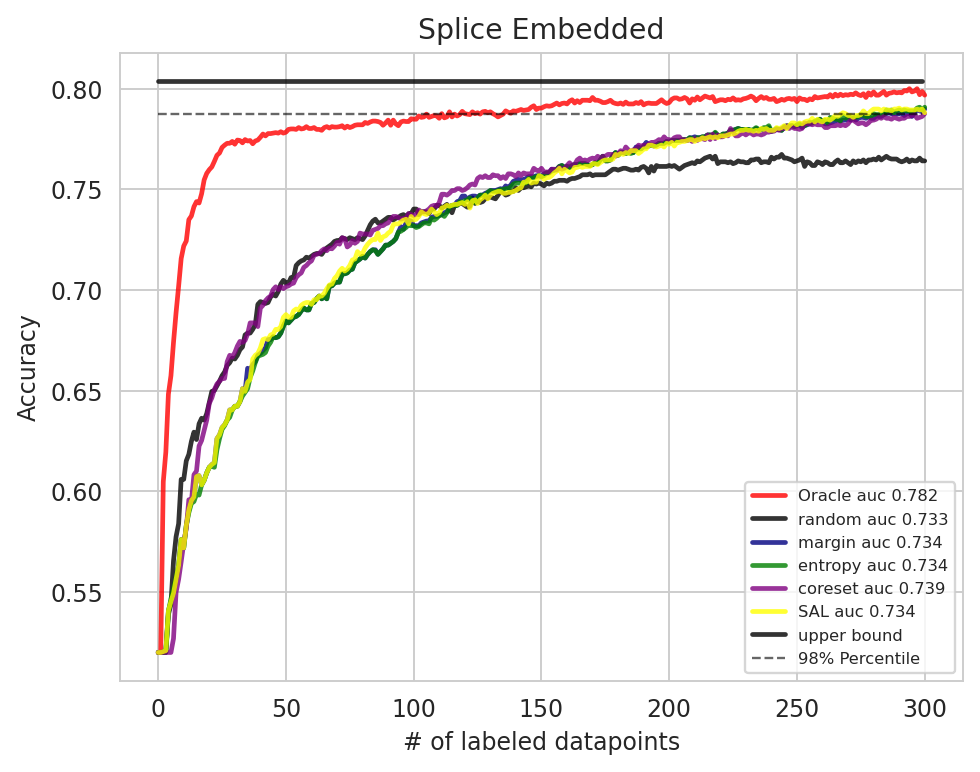
\includegraphics[width=0.8\linewidth]{img/eval_splice_embedded}
	\caption{Results for all algorithms on the pre-encoded Splice dataset}
\end{figure}
\begin{figure}[H]
\centering
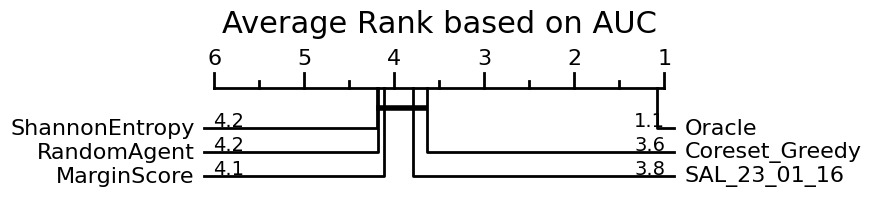
\includegraphics[width=0.8\linewidth]{img/eval_splice_embedded_cd}
\caption{Critical Difference Diagram for Splice where every restart of the algorithm is one sample for the Wilcoxon-Holm method}
\end{figure}
\begin{figure}[H]
\centering
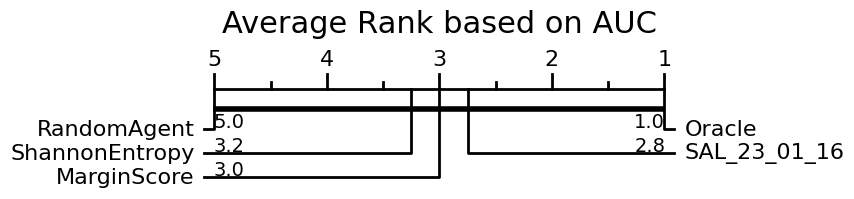
\includegraphics[width=0.8\linewidth]{img/eval_macro}
\caption{Critical Difference Diagram for Splice, DNA, USPS and Cifar10}
\end{figure}



%%%%%%%%%%%%%%%%%%%%%%%%%%%%%%%%%%%%%%%%%%%%%%%%%%%%%%%%%%%%%%%%%%%%%%%%%%%%%%%%%%
%%%%%%%%%%%%%%%%%%%%%%%%%%%%%%%%%%%%%%%%%%%%%%%%%%%%%%%%%%%%%%%%%%%%%%%%%%%%%%%%%%
\section{Ablation Studies}
\begin{itemize}
	\item Setting $\tau$ to $|\mathcal{U}|$
	\item Reduction of the test set for speed
\end{itemize}


\bibliographystyle{plain}
\bibliography{main.bib} 

\appendix

\section{Comparison of different sample sizes $\tau$}
\begin{figure}[H]
	\centering
	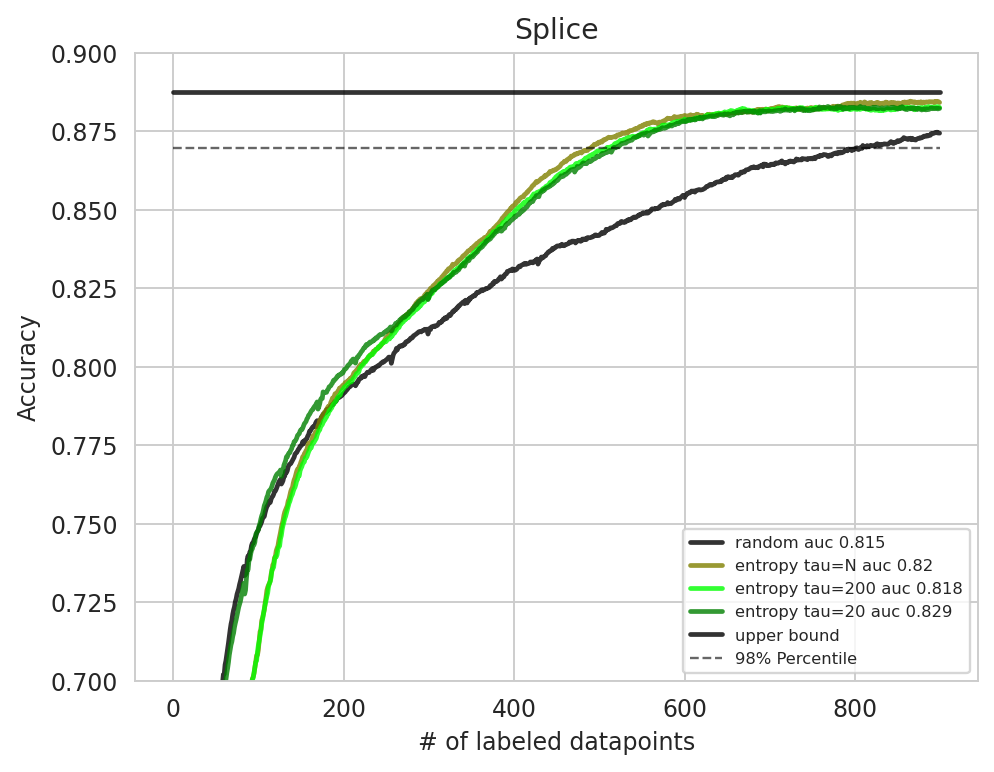
\includegraphics[width=0.7\linewidth]{img/tau_ablation.png}
\end{figure}

\end{document}